\documentclass{acm_proc_article-sp}
\usepackage{amssymb}
\usepackage[mathscr]{euscript}
\usepackage{mathtools}
\usepackage{amsmath}
\usepackage{enumerate}
\usepackage{listings}
\usepackage{tikz}
\usepackage[breaklinks]{hyperref}
\usepackage{needspace}
\usepackage{centernot}
\usetikzlibrary{positioning}

\begin{document}
\newcommand{\valueAnalysisCPA}{ValueAnalysisCPA}
\newcommand{\constraintsCPA}{ConstraintsCPA}
\newcommand{\locationCPA}{LocationCPA}
\newcommand{\symbolicExecutionCPA}{SymbolicExecutionCPA}
\newcommand{\symbolicValueCPA}{SymbolicValueCPA}
\newcommand{\compositeCPA}{CompositeCPA}
\sloppy
\title{Symbolic Execution in CPAchecker}
\subtitle{}
\numberofauthors{1}
\author{
  \alignauthor
  Thomas Lemberger
  \email{lemberge@fim.uni-passau.de}
}
\maketitle

\begin{abstract}
  The value analysis of CPAchecker, a successful tool for configurable software verification, possesses high performance but is not able to handle non-deterministic values in general.
This results in a high amount of false alarms.
While counterexample checks with other analyses are currently used to mitigate this problem,
we extend the existing value analysis to allow the handling of non-deterministic values and introduce a new configurable program analysis (CPA) to track relations between such values.
Our evaluation shows that this allows analyzing programs that use non-deterministic values correctly without the need for counterexample checks.
\end{abstract}

\section{Motivation}
With the rise of ubiquitious computing, reactive software systems that constantly receive input from the outside become more and more common.
Because of their non\--func\-tio\-nal behaviour, the unreliability of testing with a finite number of test values becomes even more severe for such programs.
In constrast to this, automatic software verification offers a more reliable alternative by analyzing all possible behaviours of a program.
Configurable software verification\cite{Beyer2007} and one of its implementations CPAchecker\cite{Beyer2011} represent a recent approach to software verification that has been successful in
multiple iterations of the Competition on Software Verification (SV-COMP) \cite{SV-COMP2013} \cite{SV-COMP2014} \cite{SV-COMP2015}.

A prominent CPA used in CPAchecker is the \valueAnalysisCPA\ \cite{Beyer2013}.
While it offers high efficiency, it only tracks explicit values and cannot handle non-deterministic ones.
Consider the simple example program in Listing \ref{exProg}. Its analysis by the \valueAnalysisCPA\ is displayed in Figure \ref{exGraph}.
It can easily be seen that the non-deterministic value of $a$ cannot be handled and as such is discarded.
Because of this imprecision, necessary information about the relation between $a$ and $b$ gets lost and the safety property in Line 14 is seen as violated.

\begin{figure}[h]
\label{exProg}
\lstset{numbers=left}
\lstinputlisting[caption=A simple non-deterministic program, captionpos=b, language=C]{exampleProgram.c}
\end{figure}

This characteristic results in a high amount of false positives.
In practice, this problem is countered by the use of counterexample checks and strengthening through other CPAs.
Instead of that, we introduce symbolic values to the existing \valueAnalysisCPA\ to allow tracking of non-deterministic values.
In addition, we specify a new \constraintsCPA\ to track constraints on these symbolic values.

\begin{figure}[h]

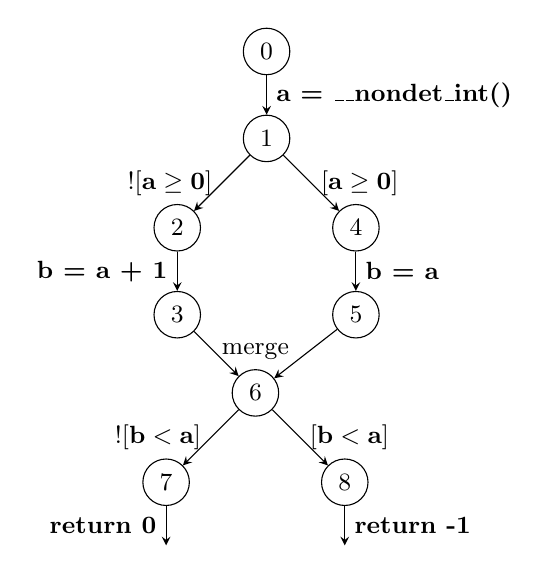
\begin{tikzpicture}[->,>=stealth, mynode/.style={circle, draw, minimum size=0.5cm}, every node/.style={font=\small}]

  \node[mynode] (0) {0};
  \node[mynode] (1) [below = 0.5cm of 0]{1};
  \node[mynode] (2) [below left = 1cm of 1]{2};
  \node[mynode] (4) [below right = 1cm of 1]{4};
  \node[mynode] (3) [below = 0.5cm of 2]{3};
  \node[mynode] (5) [below = 0.5cm of 4]{5};
  \node[mynode] (6) [below right = 0.8cm of 3, label=north:merge]{6};
  \node[mynode] (7) [below left = 1cm of 6]{7};
  \node[mynode] (8) [below right = 1cm of 6]{8};
  \coordinate[below = 0.5cm of 7] (e7);
  \coordinate[below = 0.5cm of 8] (e8);

  \path
    (0) edge node [right] {\textbf{a = \_\_nondet\_int()}} (1)
    (1) edge node [left, pos=0.5] {$\mathbf{![a \geq 0]}$} (2)
    (1) edge node [right, pos=0.5] {$\mathbf{[a \geq 0]}$} (4)
    (2) edge node [left] {\textbf{b = a + 1}} (3)
    (4) edge node [right] {\textbf{b = a}} (5)
    (3) edge (6)
    (5) edge (6)
    (6) edge node [left, pos=0.5] {$\mathbf{![b < a]}$} (7)
    (6) edge node [right, pos=0.5] {$\mathbf{[b < a]}$} (8)
    (7) edge node [left] {\textbf{return 0}} (e7)
    (8) edge node [right] {\textbf{return -1}} (e8)
  ;
\end{tikzpicture}
\label{exGraph}
\caption{Graph illustrating the analysis of the program in Listing \ref{exProg} by the \valueAnalysisCPA. The abstract state of the \valueAnalysisCPA\ is always empty as it does not track non-deterministic values. Because of this, states are merged at Location 6.}
\end{figure}

First, we will give the formal specification of a composite CPA (which we will call \symbolicExecutionCPA) using these two components. After this, an implementation of this CPA based on CPAchecker is presented. An evaluation on benchmarks taken from SV-COMP 2015 will show that the addition of symbolic value tracking allows the correct analysis of programs that could priorly not be solved by the \valueAnalysisCPA\ alone.

\Needspace{7\baselineskip}
\newcommand{\symex}{\mathbb{S}}

\newcommand{\constraints}{\mathbb{C}}
\newcommand{\location}{\mathbb{L}}
\newcommand{\composition}{\mathscr{C}}

\newcommand{\transfer}{\rightsquigarrow}
\newcommand{\gtransfer}{\overset{g}{\transfer}}
\newcommand{\strengthen}{\downarrow}

\newcommand{\valueset}{\mathscr{Z}}
\newcommand{\integerset}{\mathbb{Z}}

\newcommand{\symlattice}{\mathscr{E}}
\newcommand{\symidset}{S_I}
\newcommand{\symexpset}{S_E}

\newcommand{\constraintlattice}{\mathscr{C}}

\newcommand{\llbracket}{[\![}
\newcommand{\rrbracket}{]\!]}
\newcommand{\concretization}{\llbracket \cdot \rrbracket}
\newcommand{\lesserEqual}{\sqsubseteq}
\newcommand{\leastupperbound}{\sqcup}

\newcommand{\satisfies}{\vDash}

\section{Specification}
The symbolic execution CPA is a composite CPA of the \emph{location CPA}, the \emph{symbolic value CPA} which tracks and computes the deterministic and non-deterministic values of variables and the \emph{constraints CPA}, which tracks encountered assumptions in form of constraints for each location's variables. The formal definitions of composite CPA and location CPA are used as defined in \cite{Beyer2007}.

For the sake of formal simplicity, we assume that all values are integers and that a program only consists of assignments and assumptions.

\subsection{Symbolic value CPA}
The described CPA is an extension of the priorly mentioned value analysis CPA.
Instead of using a bottom element $\bot$, we represent an unreachable state through the absence of a valid transfer.
The symbolic value CPA is defined as
\[\symex = (D_\symex, \transfer_\symex, merge^{sep}\ stop^{sep})\]
with abstract domain $D_\symex$, transfer relation $\transfer_\symex$, merge operator $merge^{sep}$ and stop operator $stop^{sep}$.

The abstract domain $D_\symex$ is defined as
$D_\symex = (C, \symlattice, \concretization )$
with $C$ being the set of concrete program states, $\symlattice$ the semi-lattice of possible abstract states and $\concretization$ the concretization function.
%%%%%%%%%%%%%%%%%%%%%%%%%%%%
% Beginn semi-lattice definition
%%%%%%%%%%%%%%%%%%%%%%%%%%%%
\[\symlattice = (V_\symex,
                  \lesserEqual, 
                  \leastupperbound, 
                  v_\top
                )        
\]
The elements of the semi-lattice are partial functions of $V_\symex = X \rightarrow (\integerset \cup \valueset_\symex)$ mapping program variables in its definition range to concrete values of $\integerset$
or to symbolic values $\valueset_\symex = \symidset \cup \symexpset$.
$\symidset$ describes all symbolic identifiers and
$\symexpset$ is the set of all valid symbolic expressions. Each expression is a symbolic expression if at least one symbolic identifier occurs in it.
%% Old, replaced by "if at least one symbolic identifier occurs in it"
%Symbolic expressions are inductively defined as follows:
%  (1) Each expression over concrete values and symbolic identifiers is a symbolic expression, if at least one symbolic identifier occurrs.
%  (2) Each expression over symbolic expressions is a symbolic expression. Formally, this can be expressed in the following way:
%  \begin{align*}
%    \text{(1) }& a, b \in (\symidset \cup \integerset) \text{ and } \{a, b\} \cap \symidset \neq \emptyset \Rightarrow (a \circ b) \in \symexpset \\
%    \text{(2) }& c, d \in S_E \Rightarrow (c \circ d) \in \symexpset
%  \end{align*}
%using $\circ \in \{+, -, *, / , \% , \ll , \gg , \&, |, \oplus\}$.
The definition range of a function $f$ is defined as $\text{def}(f) = \{x\ | \exists y: f(x) = y\}$. The definition range of an abstract variable assignment of the type $V_\symex$ consists of all program variables $x \in X$ whose value is known, with $X$ being the set of all program variables occurring in the program. There are multiple reasons for unknown values: Uninitialized variables are unknown, but input values or calls to unknown functions and operations are, too.

To define $\lesserEqual$, we first have to define the relation between concrete and abstract states.
A concrete state $c \in C$ is \emph{compliant} to an abstract variable assignment $v$, if an arbitrary, but valid assignment of concrete values to symbolic identifiers $d: S_I \rightarrow \integerset$ exists, so that for all $x \in def(v)$ one of the following conditions is fulfilled:
(1) the abstract assignment is a concrete value that equals the value in the concrete state, that means $c(x) = v(x)$, or
(2) the abstract assignment $v(x)$ is a symbolic value that can be evaluated to $c(x)$ by replacing all occurring symbolic identifiers $i \in \symidset$ with $d(i)$.
The concretization function $\concretization$ then assigns all compliant concrete states to an abstract state $v$.

For two abstract states $v, v' \in V_\symex$, the concrete states that are covered by $v$ are a subset of the ones covered by $v'$, noted as $v \lesserEqual v'$, if all of the following conditions hold:
(1) $v'$ must only contain value assignments also present in $v$, that is $\text{def}(v') \subseteq \text{def}(v)$,
(2) $\forall x \in \text{def}(v'): v'(x) \in \integerset \Rightarrow v'(x) = v(x)$ and
(3) a bijective function $\text{alias}:\symidset \rightarrow \symidset$ exists
that maps each symbolic identifier of $\symidset$ to another symbolic identifier,
so that $\forall x \in \text{def}(v'): v'(x) \in \valueset_\symex \Rightarrow v(x)$ results from $v'(x)$ by replacing all $i \in \symidset$ occurring in $v'(x)$ with $\text{alias}(i)$.
Constraint 3 ensures that not the symbolic values themselves are compared, but their coverage of concrete states.
Consider $v = \{ (a, s1), (b, s1 + 5) \}$ and $v' = \{ (a, s2), (b, s2 + 5) \}$ with $a, b \in X$ and $s1, s2 \in S_I$. As $s1$ and $s2$ represent any possible value, $v$ represents the same amount of concrete states as $v'$, that is all $c \in C$ with $c(b) = c(a) + 5$ and an arbitrary $c(a)$. Because of this, $v' \lesserEqual v$ (and in this case even $v \lesserEqual v'$).

Note that $v' \lesserEqual v \Rightarrow \llbracket v' \rrbracket \subseteq \llbracket v \rrbracket$,
but $\llbracket v' \rrbracket \subseteq \llbracket v \rrbracket \centernot\Rightarrow v' \lesserEqual v$.

The join $\leastupperbound$ holds the least upper bound of two lattice elements $v, v' \in V_\symex$ with
  \[ (v \leastupperbound v')(x) = v(x) \text{ for all } x \in \text{def}(v) \cap\ \text{def}(v') \text{ and } v(x) = v'(x) \text{.} \]
The top element of $\symlattice$ is defined as $v_\top = \{\}$, i.e. no known assignments exist.
%%%%%%%%%%%%%%%%%%%%%%%%%%%%
% Ende semi-lattice definition
% Fortsetzung domain definition
%%%%%%%%%%%%%%%%%%%%%%%%%%%%

% Ende Domaene - Anfang Uebergangsfkt
The transfer relation $\transfer_\symex$ contains the transfer $v \gtransfer v''$, if one of the following conditions is true:
    \begin{enumerate}[1.]
      \item $g = (l, assume(p), l')$, $\phi (p, v)$ is satisfiable and:
        \[
          v''(x) = \begin{dcases}
            c    & \parbox[t]{.25\textwidth}{if $c$ only satisfying assignment for $\phi (p, v)$ and $x \notin$ def$(v)$}\\
            y    & \parbox[t]{.25\textwidth}{if $x \notin \text{def}(v)$ and $x$ appears in $p$. $y \in S_I$ and $y$ is a new value that has not been used in any other state before}\\
            v(x) & \text{otherwise}              
          \end{dcases}
        \]
        with \[\phi (p, v) := p \wedge (\displaystyle\bigwedge_{x \in \text{def}(v),\atop {v(x) \in \integerset}} x = v(x))\]

        Note: $\phi$ performs an over-approximation, as only variables $x \in \text{def}(v)$ with an explicit value are considered.

      \item $g = (l, w := e, l')$ and:
        \[
          v''(x) = \begin{dcases}
            eval(e, v') & \text{if $x = w$} \\
            v'(x)       & \text{if $x \in$ def$(v)$}
          \end{dcases}
        \]
      with \[
         v'(x) = \begin{dcases}
            y    & \parbox[t]{.25\textwidth}{if $x \notin \text{def}(v)$ and $x$ appears in $e$. $y \in S_I$ and $y$ is a new value that has not been used in any other state before}\\
            v(x) & \text{if $x \in$ def$(v)$}
          \end{dcases}
      \]
      and $eval(e, v')$ defined as the evaluation of an expression $e$ with the given assignment.
      If any symbolic value occurs in $v(e)$, it is only partially evaluated. In this case, $eval(e, v') \in \valueset_\symex$.

      \item $v'' = v_\top$.
    \end{enumerate}
The merge operator $\text{merge}^{sep}$ is defined as $\text{merge}^{sep}(e, e') = e'$.
That means no merge is performed for different value states at the same location.
The stop operator $\text{stop}^{sep}$ considers every state of the reached set independently when checking for coverage.
It is defined as $\text{stop}^{sep}(e, R) = \exists e' \in R: e \lesserEqual e'$.
%%%%%%%%%%%%%%%%%%%%%%%%%%%%%%%%%%%%%%%%%%%%%%%%%%%%%%%%%%%%%%%%%%%%%%%%%%%%%%%%%%%%%%%%%%%%%%%%%%%%%%%%%%%%%%%%%%%%%%%
%%% Beginn ConstraintsCPA
%%%%%%%%%%%%%%%%%%%%%%%%%%%%%%%%%%%%%%%%%%%%%%%%%%%%%%%%%%%%%%%%%%%%%%%%%%%%%%%%%%%%%%%%%%%%%%%%%%%%%%%%%%%%%%%%%%%%%%%
\subsection{Constraints CPA}

The constraints CPA is a CPA \[\constraints = (D_\constraints, \transfer_\constraints, merge^{sep}, stop^{sep})\] that tracks constraints (i.e. boolean formulas) on variables that are created by assume edges.
The abstract domain $D_\constraints$ is defined by 
\[D_\constraints = (C, \constraintlattice, \concretization)\]
with concrete states $C$, the semi-lattice $\constraintlattice$ and concretization function $\concretization$.

The abstract states described by $\constraintlattice = (2^\gamma, \lesserEqual, \leastupperbound, \top)$ consist of constraints of $\gamma$.
$\gamma$ contains all possible boolean expressions over $\integerset \cup \valueset_\symex$, including symbolic expressions.
An abstract state $a \in \constraintlattice$ is interpreted as the conjunction of all its constraints.
%% Redundant with "all boolean expressions
%This can be expressed in the following formal way:
% \begin{align*}
%   \gamma = \gamma_B  \cup \{!a\ |\ a \in \gamma_B\}\\
%   \text{with } \gamma_B = \{a \circ b\ |\ a, b \in \symlattice\} \text{ and } \circ \in \{ ==, <, \leq , >, \geq \}\text{.}$
% \end{align*}

For two given states $a, a' \in \constraintlattice$, state $a$ is lesser than or equal to $a'$, if a bijective funtion $\text{alias}: \symidset \rightarrow \symidset$ exists, so that $a'' \subseteq a$ with $a''$ resulting from $a'$ by replacing all symbolic identifiers $i \in \symidset$ occurring in constraints of $a'$ with $\text{alias}(i)$.

The concretization function $\concretization$ maps an abstract state to all concrete states that satisfy this abstract state's constraints.
        \[ \llbracket a \rrbracket = \{ c \in C |\ c \satisfies \displaystyle\bigwedge_{\varphi \in a} \varphi \} \]
        Note: We assume that the empty conjunction represents true, that means $\displaystyle\bigwedge_{\varphi \in \{\}} \varphi = true$.

Constraint CPA's transfer relation $\transfer_\constraints$ contains the transfer $a \gtransfer_\constraints a'$ if one of the following conditions is fulfilled:
(1) $g = (l, assume(p), l')$, $a' = a \cup {p}$ and $a$ does not contain any variable $x \in X$
(By specifying that $a$ must not contain any variable we enforce that variables are always replaced by concrete (explicit or symbolic) values through strengthening), or
(2) $a' = a$ otherwise.

As $p$ is only added as a constraint if no variable of $X$ occurs in $a$, all resulting states of this transfer relation will be satisfiable, unless $p$ is a contradiction ($a \neq a$, for instance). Because of this, we completely disregard checking for satisfiability of constraints here.
Instead, we rely on satisfiability checks during strengthening by other CPAs.
In the following we will use the priorly defined symbolic value CPA to replace newly added constraints' variables with values and check for the whole state's satisfiability.

%%%%%%%%%%%%%%%%%%%%%%%%%%%%%%%%%%%%%%%%%%%%%%%%%%%%%%%%%%%%%%%%%%%%%%%%%%%%%%%%%%%%%%%%%%%%%%%%%%%%%%%%%%%%%%%%%%%%%%%
%%% Beginn Composition
%%%%%%%%%%%%%%%%%%%%%%%%%%%%%%%%%%%%%%%%%%%%%%%%%%%%%%%%%%%%%%%%%%%%%%%%%%%%%%%%%%%%%%%%%%%%%%%%%%%%%%%%%%%%%%%%%%%%%%%
\subsection{Composition of CPAs}
$\composition_{\location\symex\constraints} = (\location, \symex, \constraints, \transfer_x, merge^{sep}, stop^{sep})$ is the composite CPA of a location CPA and the priorly defined symbolic value CPA and constraints CPA.
The transfer relation \[\transfer_x : D_\location \times D_\symex \times D_\constraints \rightarrow D_\location \times D_\symex \times D_\constraints\] contains
the transfer $(l, v, a) \gtransfer_x (l', v', a'')$ if 
            $l \gtransfer_\location l'$,
            $v \gtransfer_\symex v'$ and
            $a \gtransfer_\constraints a'$ and
            if the strengthen operation $\strengthen_{\constraints, \symex}$ is defined for $a'$ and $v'$ with
            $\strengthen_{\constraints, \symex} (a', v') = a''$.

The strengthen operator $\strengthen_{\constraints, \symex} : \constraints \times \symex \rightarrow \constraints$ uses the value assignment $v(x)$ of the given second operand to replace variables of the latest, unstrengthened constraint of the given constraints state. This way, meaningful constraints are created that show relations between symbolic values and can be checked for satisfiability.

$\strengthen_{\constraints, \symex} (a, v) = a'$ is defined if $a'$ is the result of replacing all program variables $x \in X$ occurring in $a$ with $v(x)$ and if $\displaystyle\bigwedge_{\varphi \in a'} \varphi$ is satisfiable.

\begin{figure*}

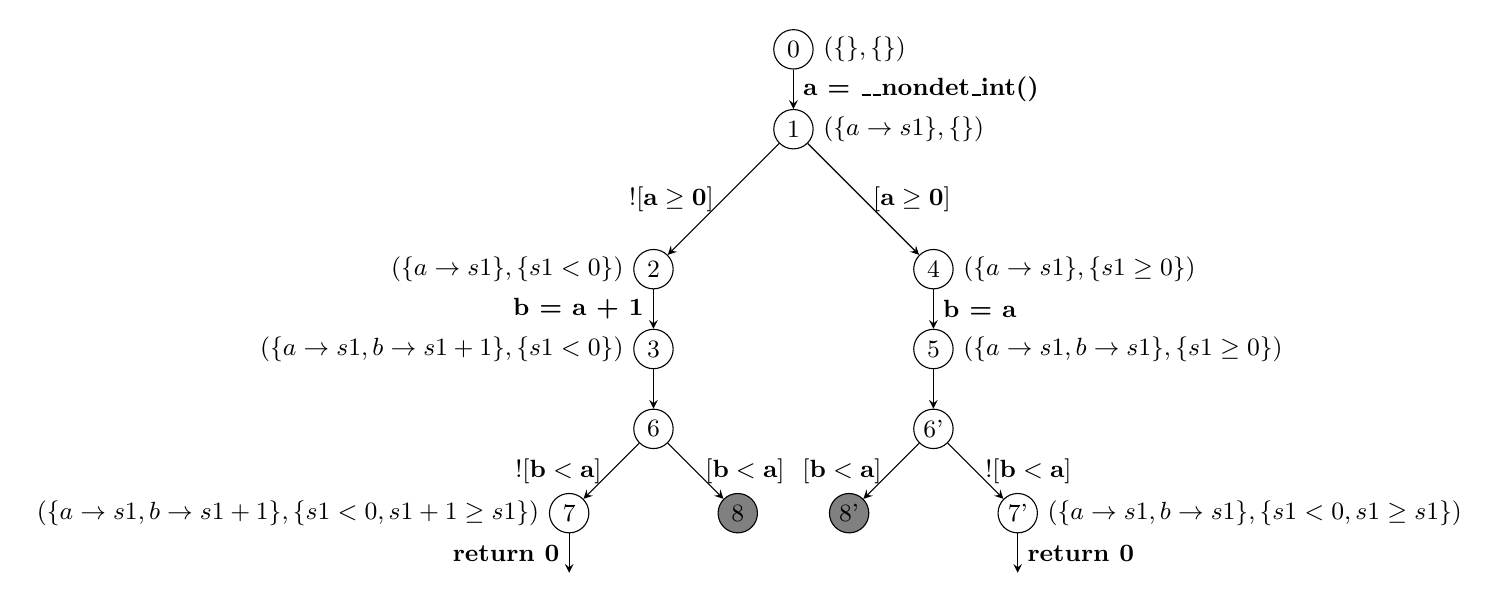
\begin{tikzpicture}[->,>=stealth, mynode/.style={circle, draw, minimum size=0.5cm, inner sep =0pt}, every node/.style={font=\small}]

  \node[mynode] (0) [label=0:{$(\{\}, \{\})$}]{0};
  \node[mynode] (1) [below = 0.5cm of 0, label=0:{$(\{a \rightarrow s1\}, \{\})$}]{1};
  \node[mynode] (2) [below left = 2cm of 1, label=west:{$(\{a \rightarrow s1\}, \{s1 < 0\})$}]{2};
  \node[mynode] (4) [below right = 2cm of 1, label=0:{$(\{a \rightarrow s1\}, \{s1 \geq 0\})$}]{4};
  \node[mynode] (3) [below = 0.5cm of 2, label=west:{$(\{a \rightarrow s1, b \rightarrow s1+1\}, \{s1 < 0\})$}]{3};
  \node[mynode] (5) [below = 0.5cm of 4, label=0:{$(\{a \rightarrow s1, b \rightarrow s1 \}, \{s1 \geq 0\})$}]{5};
  \node[mynode] (6) [below = 0.5cm of 3]{6};
  \node[mynode] (6n) [below = 0.5cm of 5]{6'};
  \node[mynode] (7) [below left = 1cm of 6, label=west:{$(\{a \rightarrow s1, b \rightarrow s1+1\}, \{s1 < 0, s1+1 \geq s1\})$}]{7};
  \node[mynode] (8) [below right = 1cm of 6, fill=gray]{8};
  \node[mynode] (8n) [below left = 1cm of 6n, fill=gray]{8'};
  \node[mynode] (7n) [below right = 1cm of 6n, label=0:{$(\{a \rightarrow s1, b \rightarrow s1\}, \{s1 < 0, s1 \geq s1\})$}]{7'};
  \coordinate[below = 0.5cm of 7] (e7);
  \coordinate[below = 0.5cm of 7n] (e7n);

  \path
    (0) edge node [right] {\textbf{a = \_\_nondet\_int()}} (1)
    (1) edge node [left, pos=0.5] {$\mathbf{![a \geq 0]}$} (2)
    (1) edge node [right, pos=0.5] {$\mathbf{[a \geq 0]}$} (4)
    (2) edge node [left] {\textbf{b = a + 1}} (3)
    (4) edge node [right] {\textbf{b = a}} (5)
    (3) edge (6)
    (5) edge (6n)
    (6) edge node [left, pos=0.5] {$\mathbf{![b < a]}$} (7)
    (6) edge node [right, pos=0.5] {$\mathbf{[b < a]}$} (8)
    (6n) edge node [left, pos=0.5] {$\mathbf{[b < a]}$} (8n)
    (6n) edge node [right, pos=0.5] {$\mathbf{![b < a]}$} (7n)
    (7) edge node [left] {\textbf{return 0}} (e7)
    (7n) edge node [right] {\textbf{return 0}} (e7n)
  ;
\end{tikzpicture}
\caption{Analysis of the program in Listing \ref{exProg} by the symbolic execution CPA. The locations reported as unreachable are tinted grey. The state is provided as a tuple at each relevant node, the first element being the state of $\symex$, the second of $\constraints$. The state of the location CPA can be derived from the node's numbers.}
\label{constGraph}
\end{figure*}

An analysis of the previous test program using symbolic execution can be seen in Figure \ref{constGraph}. 
By storing information about the relationship of variables $a$ and $b$, the CPA can derive at location 6/6' that $b$ can't be smaller than $a$.

\Needspace{7\baselineskip}
\section{Evaluation}
The specified CPA was implemented in CPAchecker\cite{Beyer2011} using the existing CompositeCPA and LocationCPA.
The existing ValueAnalysisCPA  was extended to fulfil the specification of our symbolic value CPA,
while the constraints CPA was implemented as a new, own CPA. To check the satisfiability of constraints, an external SAT checker is used. For these benchmarks, MathSAT5 is used with the bitvector theory, encoding float values as floats.
The analysis is part of CPAchecker's trunk since revision 16052 and can be activated by using the configuration \texttt{valueAnalysis-symbolic}. As development is ongoing, the current revision at the time of this writing, that is 16433, was chosen for benchmarks.

Benchmarks were performed on a subset of the SV-COMP 2015 test set, excluding sets CPAchecker's ValueAnalysisCPA has no competency in.
These excluded sets are namely "Concurrency", "Memory Safety", "Recursive" and "Termination". An overview of all test sets can be found at \cite{SV15Benchmark}.
Tests were executed on Intel Xeon E7-4870 machines at 2.40GHz with a memory limit of 15GB and a time limit of 900 seconds.

All benchmark results are available at \url{https://github.com/leostrakosch/symbolicValueAnalysis/tree/master/benchmarks}

Figure \ref{tab:diff} shows the performance of the default ValueAnalysisCPA without counterexample-guided abstraction refinement (CEGAR, \cite{XXX}) or counterexample checks next to the performance of our symbolic execution configuration. The category "timeouts" does not only include timeouts, but also two StackOverflowExceptions that resulted from long symbolic expressions. Such expressions can be generated by long loops, but are uncommon.
Generally speaking, basic value analysis easily outperforms symbolic execution in numbers.
Lots of timeouts occur due to
(a) path explosion, an exponential increase in possible paths based on the number of branches (that is if-statements and loops) as a result of the low level of abstraction of symbolic execution, and
(b) the bad performance of SAT checks with a large number of variables and arithmetic operations like non-linear multiplication.
Path explosion can easily be illustrated when looking at the algorithm statistics of a simple program using multiple if- and goto-statements (Namely: XXX)
While basic value analysis only needs about 3500 iterations to find a possible error, with the biggest waitlist consisting of 14 entries,
analysis with symbolic execution needs over 25000 iterations with the biggest waitlist consisting of almost 530 states.
In addition to this enormous growth in iterations, SAT checks are responsible for up to 95\% of CPU time in analyses of programs that are \emph{not} specifically constructed for challenging SAT checkers.

Despite this reduced speed, symbolic execution's ability to track non-deterministic values allows it to get a correct result in 41 cases in which value analysis does not. In eight of these value analysis receives timeouts, and in 33 value analysis provides a false positive. Symbolic execution does never produce a false result when value analysis produces a correct one.
\begin{figure}
\begin{tabular}{| r || r | r | r |}
\hline
        & Value & SymEx & Overall \\ \hline
correct                & 1994 &  833 & 3038 \\ \hline
true positives         &  631 &  322 &  802 \\ \hline
true negatives         & 1363 &  153 & 2236 \\ \hline
unique true positives  &  318 &    8 &    - \\ \hline
unique true negatives  & 1243 &   33 &    - \\ \hline
false positives        &  271 &   52 &    - \\ \hline
unique false positives &  220 &    5 &    - \\ \hline
false negatives        &    0 &    0 &    - \\ \hline 
timeouts               &  662 & 2451 &    - \\ \hline
errors                 &  111 &   56 &    - \\ \hline
\end{tabular}
\label{tab:diff}
\caption{Result of runs of value analysis (Value) and symbolic execution (SymEx) on SV-COMP 2015 test sets.
  "true positive" represents a found error in a program with an error,
  "true negative" represents no found error in a program without errors.}
\end{figure}

When using a timelimit of 1800 seconds, symbolic execution is able to compute 14 more results than with a timelimit of 900 seconds, of which eleven are correct.

Of these long-taking runs, five are the result of path explosion,
while the other nine only consist of few iterations, but contain expressions resulting in long-taking SAT checks, namely bitvector computations, non-deterministic floats and multiplications.

Some of these performance issues can be improved by using another theory in SAT checks.
By using an integer theory instead of bitvector, runtime can be decreased by up to 50\%, but results in a worse overall performance.
The use of integer results in an unsound analysis, too. Figure \ref{bitvecIntComp} shows the difference between the use of a bitvector theory with floats and the use of an integer theory.
\begin{figure}
\begin{tabular}{| r || r | r |}
\hline
& Bitvector theory & Integer theory \\ \hline
correct         &  475 &  461 \\ \hline
false positives &   56 &   97 \\ \hline
false negatives &    0 &    6 \\ \hline
timeouts        & 2450 & 2417 \\ \hline
errors          &   56 &   56 \\ \hline
                & & \\ \hline
\end{tabular}
\caption{Results of symbolic execution CPA using bitvector theory with floats and integer theory on SV-COMP 2015 test sets.}
\label{bitvecIntComp}
\end{figure}

\section{Conclusion}
By extending the existing ValueAnalysisCPA with the ability to track non-deterministic values and the introduction of the new ConstraintsCPA,
we were able to drastically reduce the number of falsely positive analysis results of value analysis without the need for counterexample checks.
As this is only a very basic implementation, a big amount of potential exists.

When choosing a SMT theory,
it must be considered whether to trade performance for precision depending on the underlying program's use of floats and bitwise operations known.
To decrease runtime without a loss of precision, the problem of path explosion should be tackled.
A valid approach to this could be CEGAR, which is already implemented for the ValueAnalysisCPA as described in \cite{Beyer2012}.
By resolving the problem of path explosion, the number of iterations and as such also the number of SAT checks could be decreased, while keeping our high level of precision.
This should be the main focus of future work.


\bibliographystyle{acm}
\bibliography{bib}

\end{document}
